% Options for packages loaded elsewhere
\PassOptionsToPackage{unicode}{hyperref}
\PassOptionsToPackage{hyphens}{url}
\PassOptionsToPackage{dvipsnames,svgnames,x11names}{xcolor}
%
\documentclass[
  letterpaper,
  DIV=11,
  numbers=noendperiod]{scrartcl}

\usepackage{amsmath,amssymb}
\usepackage{iftex}
\ifPDFTeX
  \usepackage[T1]{fontenc}
  \usepackage[utf8]{inputenc}
  \usepackage{textcomp} % provide euro and other symbols
\else % if luatex or xetex
  \usepackage{unicode-math}
  \defaultfontfeatures{Scale=MatchLowercase}
  \defaultfontfeatures[\rmfamily]{Ligatures=TeX,Scale=1}
\fi
\usepackage{lmodern}
\ifPDFTeX\else  
    % xetex/luatex font selection
\fi
% Use upquote if available, for straight quotes in verbatim environments
\IfFileExists{upquote.sty}{\usepackage{upquote}}{}
\IfFileExists{microtype.sty}{% use microtype if available
  \usepackage[]{microtype}
  \UseMicrotypeSet[protrusion]{basicmath} % disable protrusion for tt fonts
}{}
\makeatletter
\@ifundefined{KOMAClassName}{% if non-KOMA class
  \IfFileExists{parskip.sty}{%
    \usepackage{parskip}
  }{% else
    \setlength{\parindent}{0pt}
    \setlength{\parskip}{6pt plus 2pt minus 1pt}}
}{% if KOMA class
  \KOMAoptions{parskip=half}}
\makeatother
\usepackage{xcolor}
\setlength{\emergencystretch}{3em} % prevent overfull lines
\setcounter{secnumdepth}{-\maxdimen} % remove section numbering
% Make \paragraph and \subparagraph free-standing
\ifx\paragraph\undefined\else
  \let\oldparagraph\paragraph
  \renewcommand{\paragraph}[1]{\oldparagraph{#1}\mbox{}}
\fi
\ifx\subparagraph\undefined\else
  \let\oldsubparagraph\subparagraph
  \renewcommand{\subparagraph}[1]{\oldsubparagraph{#1}\mbox{}}
\fi


\providecommand{\tightlist}{%
  \setlength{\itemsep}{0pt}\setlength{\parskip}{0pt}}\usepackage{longtable,booktabs,array}
\usepackage{calc} % for calculating minipage widths
% Correct order of tables after \paragraph or \subparagraph
\usepackage{etoolbox}
\makeatletter
\patchcmd\longtable{\par}{\if@noskipsec\mbox{}\fi\par}{}{}
\makeatother
% Allow footnotes in longtable head/foot
\IfFileExists{footnotehyper.sty}{\usepackage{footnotehyper}}{\usepackage{footnote}}
\makesavenoteenv{longtable}
\usepackage{graphicx}
\makeatletter
\def\maxwidth{\ifdim\Gin@nat@width>\linewidth\linewidth\else\Gin@nat@width\fi}
\def\maxheight{\ifdim\Gin@nat@height>\textheight\textheight\else\Gin@nat@height\fi}
\makeatother
% Scale images if necessary, so that they will not overflow the page
% margins by default, and it is still possible to overwrite the defaults
% using explicit options in \includegraphics[width, height, ...]{}
\setkeys{Gin}{width=\maxwidth,height=\maxheight,keepaspectratio}
% Set default figure placement to htbp
\makeatletter
\def\fps@figure{htbp}
\makeatother
\newlength{\cslhangindent}
\setlength{\cslhangindent}{1.5em}
\newlength{\csllabelwidth}
\setlength{\csllabelwidth}{3em}
\newlength{\cslentryspacingunit} % times entry-spacing
\setlength{\cslentryspacingunit}{\parskip}
\newenvironment{CSLReferences}[2] % #1 hanging-ident, #2 entry spacing
 {% don't indent paragraphs
  \setlength{\parindent}{0pt}
  % turn on hanging indent if param 1 is 1
  \ifodd #1
  \let\oldpar\par
  \def\par{\hangindent=\cslhangindent\oldpar}
  \fi
  % set entry spacing
  \setlength{\parskip}{#2\cslentryspacingunit}
 }%
 {}
\usepackage{calc}
\newcommand{\CSLBlock}[1]{#1\hfill\break}
\newcommand{\CSLLeftMargin}[1]{\parbox[t]{\csllabelwidth}{#1}}
\newcommand{\CSLRightInline}[1]{\parbox[t]{\linewidth - \csllabelwidth}{#1}\break}
\newcommand{\CSLIndent}[1]{\hspace{\cslhangindent}#1}

\usepackage{booktabs}
\usepackage{longtable}
\usepackage{array}
\usepackage{multirow}
\usepackage{wrapfig}
\usepackage{float}
\usepackage{colortbl}
\usepackage{pdflscape}
\usepackage{tabu}
\usepackage{threeparttable}
\usepackage{threeparttablex}
\usepackage[normalem]{ulem}
\usepackage{makecell}
\usepackage{xcolor}
\KOMAoption{captions}{tableheading}
\makeatletter
\makeatother
\makeatletter
\makeatother
\makeatletter
\@ifpackageloaded{caption}{}{\usepackage{caption}}
\AtBeginDocument{%
\ifdefined\contentsname
  \renewcommand*\contentsname{Table of contents}
\else
  \newcommand\contentsname{Table of contents}
\fi
\ifdefined\listfigurename
  \renewcommand*\listfigurename{List of Figures}
\else
  \newcommand\listfigurename{List of Figures}
\fi
\ifdefined\listtablename
  \renewcommand*\listtablename{List of Tables}
\else
  \newcommand\listtablename{List of Tables}
\fi
\ifdefined\figurename
  \renewcommand*\figurename{Figure}
\else
  \newcommand\figurename{Figure}
\fi
\ifdefined\tablename
  \renewcommand*\tablename{Table}
\else
  \newcommand\tablename{Table}
\fi
}
\@ifpackageloaded{float}{}{\usepackage{float}}
\floatstyle{ruled}
\@ifundefined{c@chapter}{\newfloat{codelisting}{h}{lop}}{\newfloat{codelisting}{h}{lop}[chapter]}
\floatname{codelisting}{Listing}
\newcommand*\listoflistings{\listof{codelisting}{List of Listings}}
\makeatother
\makeatletter
\@ifpackageloaded{caption}{}{\usepackage{caption}}
\@ifpackageloaded{subcaption}{}{\usepackage{subcaption}}
\makeatother
\makeatletter
\@ifpackageloaded{tcolorbox}{}{\usepackage[skins,breakable]{tcolorbox}}
\makeatother
\makeatletter
\@ifundefined{shadecolor}{\definecolor{shadecolor}{rgb}{.97, .97, .97}}
\makeatother
\makeatletter
\makeatother
\makeatletter
\makeatother
\ifLuaTeX
  \usepackage{selnolig}  % disable illegal ligatures
\fi
\IfFileExists{bookmark.sty}{\usepackage{bookmark}}{\usepackage{hyperref}}
\IfFileExists{xurl.sty}{\usepackage{xurl}}{} % add URL line breaks if available
\urlstyle{same} % disable monospaced font for URLs
\hypersetup{
  pdftitle={Estimating Future Traffic Volumes at the I-15 Interchange at Main Street in Payson, Utah},
  pdfauthor={Hayden Atchley; Adam Hill; Matthew Davis; Sam Runyan},
  colorlinks=true,
  linkcolor={blue},
  filecolor={Maroon},
  citecolor={Blue},
  urlcolor={Blue},
  pdfcreator={LaTeX via pandoc}}

\title{Estimating Future Traffic Volumes at the I-15 Interchange at Main
Street in Payson, Utah}
\author{Hayden Atchley \and Adam Hill \and Matthew Davis \and Sam
Runyan}
\date{20 November 2023}

\begin{document}
\maketitle
\ifdefined\Shaded\renewenvironment{Shaded}{\begin{tcolorbox}[breakable, boxrule=0pt, sharp corners, borderline west={3pt}{0pt}{shadecolor}, interior hidden, enhanced, frame hidden]}{\end{tcolorbox}}\fi

In the previous reports, existing and design conditions were tested
using current volumes (Atchley et al. 2023a) (Atchley et al. 2023b).
However, it will be necessary to test these conditions using projected
volumes from 2022 to the 2050 horizon year. The existing condition will
be tested under future volumes to test a ``no build'' scenario, and the
design conditions will be tested under future volumes to test a
``build'' scenario.

The projected volumes will be created using a traffic simulation program
called Multi-Agent Transport Simulation (MATSim) (Association 2023).
This program simulates individual travelers in a transportation network
and ``trains'' them to find the optimal path during their tour by
running the simulation through multiple iterations. Individual travelers
can be counted at the study area to obtain traffic volumes. This allows
some flexibility to be able to model future traffic volumes as explained
in the following sections.

This memorandum includes information of the population creation model,
the MATSim network, forecasted volumes, and the resulting turning counts
from the MATSim model.

\hypertarget{population-creation}{%
\section{Population Creation}\label{population-creation}}

The population of Payson, UT was synthetically created using MATSim.
Assumptions used for population development are detailed in this
section, including the creation and assignment of discretionary,
non-discretionary, and home-based tours. These tours include a list of
destinations and arrival times for each event. All trips are assigned to
a personal vehicle, but the route that the vehicle takes is derived
through a best fit algorithm.

Tour type was randomly assigned by the distribution included in
Table~\ref{tbl-tourtypedist}. These values were derived from the 2017
National Household Travel Survey ({``National {Household} {Travel}
{Survey}''} 2017) for metropolitan areas between one and three million
people. Workers and non-workers were created with a probability of 42\%
of the total population being a worker.

``Home'' assignments were created on a normal distribution with the mean
and standard deviation for longitude and latitude defined in
Table~\ref{tbl-locdist}. These distributions were also used for the
creation of non-mandatory trips for both Mandatory and Non-Mandatory
tour creation. Creation of Table~\ref{tbl-locdist} was conducted using
population weighted block groups from the 2010 census ({``United
{States} {Census}- {Files}''} 2010).

\hypertarget{tbl-tourtypedist}{}
\begin{longtable}[]{@{}llll@{}}
\caption{\label{tbl-tourtypedist}Tour Type Distribution}\tabularnewline
\toprule\noalign{}
PERSON TYPE & HOME & MANDATORY & NON-MANDATORY \\
\midrule\noalign{}
\endfirsthead
\toprule\noalign{}
PERSON TYPE & HOME & MANDATORY & NON-MANDATORY \\
\midrule\noalign{}
\endhead
\bottomrule\noalign{}
\endlastfoot
Non-Worker & 0.229 & 0.165 & 0.605 \\
Worker & 0.083 & 0.632 & 0.285 \\
\end{longtable}

\hypertarget{tbl-locdist}{}
\begin{longtable}[]{@{}llll@{}}
\caption{\label{tbl-locdist}Location Distributions}\tabularnewline
\toprule\noalign{}
lat & lon & lat\_sd & lon\_sd \\
\midrule\noalign{}
\endfirsthead
\toprule\noalign{}
lat & lon & lat\_sd & lon\_sd \\
\midrule\noalign{}
\endhead
\bottomrule\noalign{}
\endlastfoot
40.03375 & -111.7362 & 0.0105619 & 0.0135612 \\
\end{longtable}

Non-mandatory trip tours are comprised of one to three discretionary
trips. These destinations were created on the normal distributions as
described in Table~\ref{tbl-locdist}. Start and end times for the tour
were constrained to be between 6 am and 10 pm. Each subsequent activity
begins at a random time after the previous one (Mandatory activities
begin between 7 am and 9 am and end between 4 pm and 6 pm). End times
were similarly assigned but with a correction factor to ensure that
trips end by 10 pm.

A random distribution was developed to determine if trips were
concurrent, or if users returned to their ``home'' location in between.
If a single trip had been taken, there was a 40\% that they would return
home, if two trips, 60\%, and if three trips, then 80\%. This
distribution was created to reflect personal opinions of the likelihood
of concurrent trips after a given number of previous concurrent trips.
Once all trips or the day ended, whichever came first, the non-mandatory
tour was completed.

Mandatory trip tours comprise of a trip to I-15 northbound (NB) or
southbound (SB) and a possible discretionary activity on the way to the
``home'' location. Coordinates were selected on the north and southern
ends of the model to assign individuals to travel in such direction
either going north to Spanish Fork/Provo and beyond, or south to
Santaquin/Nephi and beyond. A random distribution assigned 95\% of all
mandatory trips northbound. Start time for mandatory trips were between
7-9 am. End times were between 4-6 pm. Mandatory trip tours were given a
50\% chance to complete a discretionary trip. Start times for that trip
were within 1 hour of the mandatory trip end time with a duration of 30
minutes. Discretionary trip destinations were selected along a normal
distribution from Table~\ref{tbl-locdist}. All discretionary trips
originated from the mandatory trip location and ended at the ``home''
location. After returning ``home'' the mandatory tour was completed.

\hypertarget{matsim-network}{%
\section{MATSim Network}\label{matsim-network}}

The team was provided with a network for the Payson MATSim model that
roughly modeled the actual roadway network in and around Payson, UT.
Using this network means that the paths that agents take should be close
to available paths in Payson, UT. Attributes included in each roadway
link were speed, number of lanes, annual average daily traffic (AADT)
and capacity. Figure~\ref{fig-network} displays the MATSim network
overlayed on a map of Payson, UT.

\begin{figure}

{\centering \includegraphics[width=5.72917in,height=\textheight]{matsim/network.png}

}

\caption{\label{fig-network}MATSim Payson network}

\end{figure}

\hypertarget{population-projections}{%
\section{Population Projections}\label{population-projections}}

The population for Payson, UT in 2050 was projected using a growth rate
based on Utah County growth over the same time period. Based on numbers
from the Kem C. Gardner Policy Institute, the population of Utah County
in 2022 was 702,943 and the projected population for 2050 is 1,185,679
({``State and {County} {Projections}''} 2022). This is a cumulative net
growth rate of 68.7\% from 2022 to 2050. It is important to note that
this is not a yearly compounded growth rate, but a linear growth rate
between the two populations. As Payson is in Utah County and has plenty
of room for growth, the team felt comfortable applying the Utah County
growth rate to Payson's population.

The population of Payson, UT in 2022 was 22,516, so with a 68.7\% net
growth rate, this means that the projected population of Payson, UT in
2050 is approximately 37,979 ({``{QuickFacts}: {Payson} City, {Utah}:
{Utah} {County}, {Utah}''} 2022). The traffic volumes at the study area
were projected using a growth rate derived from the MATSim model. The
MATSim model was run with the existing population size for Payson and
again with a projected population size for Payson. This allowed for a
growth rate to be calculated for each turning movement at the study
area. Rather than using the projected volumes produced by MATSim, the
growth rate was applied to the volumes produced in the VISSIM model for
existing traffic to calculate projected traffic volumes. Households are
illustrated in Figure~\ref{fig-loaded-network}.

\begin{figure}

{\centering \includegraphics[width=4.6875in,height=\textheight]{matsim/Home.jpg}

}

\caption{\label{fig-loaded-network}MATSim Loaded Payson network}

\end{figure}

Even though the traffic volumes produced by the MATSim model are
incomplete, the growth rates calculated from MATSim are reasonable to
apply to the VISSIM model as an academic exercise.

\hypertarget{results}{%
\section{Results}\label{results}}

Table~\ref{tbl-tmc} shows the calculated MATSim turning movement counts
for each intersection at the study area for 2022 and 2050. These
intersections are visualized in Figure~\ref{fig-via} and hourly traffic
patterns are shown. Intersection movement counts were collected for the
entire simulation run time due to extensive delays in the pm. The growth
rate was calculated as shown in Equation~\ref{eq-growth}.

As presented in the figure, the northern intersections exhibit a growth
of approximately 40\% from 2022 to 2050 while the southern intersections
exhibit a growth of approximately 30\% from 2022 to 2050.

\begin{equation}\protect\hypertarget{eq-growth}{}{
Growth(\%)=\frac{2050-2022 \; Volumes}{2022 \; Volumes}(100\%)
}\label{eq-growth}\end{equation}

\hypertarget{tbl-tmc}{}
\begin{longtable}[]{@{}
  >{\raggedright\arraybackslash}p{(\columnwidth - 6\tabcolsep) * \real{0.2500}}
  >{\raggedright\arraybackslash}p{(\columnwidth - 6\tabcolsep) * \real{0.2500}}
  >{\raggedright\arraybackslash}p{(\columnwidth - 6\tabcolsep) * \real{0.2500}}
  >{\raggedright\arraybackslash}p{(\columnwidth - 6\tabcolsep) * \real{0.2500}}@{}}
\caption{\label{tbl-tmc}Existing and Projected Turning Movement
Counts}\tabularnewline
\toprule\noalign{}
\begin{minipage}[b]{\linewidth}\raggedright
\textbf{Intersection}
\end{minipage} & \begin{minipage}[b]{\linewidth}\raggedright
\textbf{2022 Turning Counts}
\end{minipage} & \begin{minipage}[b]{\linewidth}\raggedright
\textbf{2050 Turning Counts}
\end{minipage} & \begin{minipage}[b]{\linewidth}\raggedright
\textbf{Cumulative Growth Rates}
\end{minipage} \\
\midrule\noalign{}
\endfirsthead
\toprule\noalign{}
\begin{minipage}[b]{\linewidth}\raggedright
\textbf{Intersection}
\end{minipage} & \begin{minipage}[b]{\linewidth}\raggedright
\textbf{2022 Turning Counts}
\end{minipage} & \begin{minipage}[b]{\linewidth}\raggedright
\textbf{2050 Turning Counts}
\end{minipage} & \begin{minipage}[b]{\linewidth}\raggedright
\textbf{Cumulative Growth Rates}
\end{minipage} \\
\midrule\noalign{}
\endhead
\bottomrule\noalign{}
\endlastfoot
900 North & 5295 & 7354 & 38.9\% \\
SB Interchange & 7983 & 11101 & 39.1\% \\
NB Interchange & 8883 & 11716 & 31.9\% \\
600 North & 6806 & 8846 & 30.0\% \\
\end{longtable}

Turning movement proportions were very similar between the 2022 and 2050
models. Figure~\ref{fig-via} shows the turning movement distributions
and histograms illustrating the volume breakdowns between the 2022 and
2050 models. Generally, the distributions widen in 2050, with the pm
queues taking more than two additional hours to dissipate in the 2050
model as compared to the 2022 model (from 7pm to 9:30pm).

\begin{figure}

{\centering 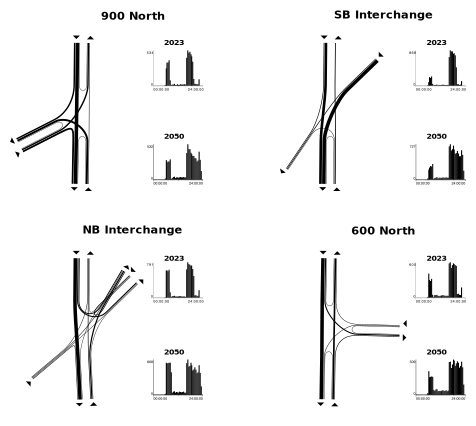
\includegraphics{figures/matsim_intersections/VIA_diagram.png}

}

\caption{\label{fig-via}Existing and projected turning movement counts.}

\end{figure}

Each segment in the network was heavily utilized as drivers looked for
the best cost path that would minimize the time and distance traveled.
The most severe congestion was present along Main St in the AM peak and
the SB I-15 corridor in the PM peak. These segments are well over
capacity. However, given the experimental nature of the methodology it
is unwise to make planning judgements from this model. The rough growth
rates collected from the model will be reviewed and implemented in
future steps.

Also, of note are Figures \ref{fig-2022-scores} and
\ref{fig-2050-scores} which illustrate that over the 200 iterations, the
model appears to converge to an equilibrium fit. The 2050 model required
more interactions to converge, but after 190 iterations were consistent
in its convergence. The 2022 model converged after 125 interactions,
likely due to the lower volumes in the network.

Figures \ref{fig-hist-2022} and \ref{fig-2050-hist} show the trip
distributions for the 200th iteration. The strong peaks at the beginning
and end of the time period reflects the stay-at-home and non-mandatory
individuals as the model treats them as starting their ``home'' trip at
6am and returning ``home'' at 10 pm. During the AM peak, drivers are
able to reach their destinations sooner, leading to a smaller number of
vehicle hours traveled. The PM peak has a significantly higher number of
vehicles hours traveled due to the higher levels of congestion.

It is possible that there may be a error in the network file that
reduced the capacity of the I-15 SB segments, leading to a inflation in
delay. The sharp bins in departures from 6-8 am and 4-6 pm illustrate
the modeling characteristics of the model as mandatory trips were forced
to leave during those time frames. Table \ldots{} shows the growth rates
applied to the existing counts that were collected for the existing
VISSIM model. OD pairs will be calculated from this data and used in the
``No-Build'' and ``Build 2050'' models for future analysis.

\begin{figure}

{\centering \includegraphics[width=\textwidth,height=3.5in]{figures/matsim/scorestats2022.png}

}

\caption{\label{fig-2022-scores}MATSim scores for 2022 model.}

\end{figure}

\begin{figure}

{\centering \includegraphics[width=\textwidth,height=3.5in]{figures/matsim/scorestats2050.png}

}

\caption{\label{fig-2050-scores}MATSim Scores for 2050 model.}

\end{figure}

\begin{figure}

{\centering \includegraphics[width=\textwidth,height=3.5in]{figures/matsim/200.legHistogram_all2022.png}

}

\caption{\label{fig-hist-2022}Trip histogram for 2022 model.}

\end{figure}

\begin{figure}

{\centering \includegraphics[width=\textwidth,height=3.5in]{figures/matsim/200.legHistogram_all2050.png}

}

\caption{\label{fig-2050-hist}Trip histogram for 2050 model.}

\end{figure}

\hypertarget{conclusions}{%
\section{Conclusions}\label{conclusions}}

MATSim provides a method for creating turning counts even with limited
prediction models. As an academic exercise, these results and growth
rates will be used to forecast growth in VISSIM to provide limited
recommendations for future growth at the I-15 interchange at Main St in
Payson, Utah.

\hypertarget{references}{%
\section{References}\label{references}}

\hypertarget{refs}{}
\begin{CSLReferences}{1}{0}
\leavevmode\vadjust pre{\hypertarget{ref-MATSim}{}}%
Association, MATSim. 2023. {``Multi-Agent Transport Simulation.''}
\url{https://www.matsim.org/}.

\leavevmode\vadjust pre{\hypertarget{ref-design}{}}%
Atchley, Hayden, Adam Hill, Samuel Runyan, and Matthew Davis. 2023a.
{``{Redesign} of the {I}-15 {Interchange} at {Main} {Street} in
{Payson}, {Utah}.''} Memorandum. BYU CE 662.

\leavevmode\vadjust pre{\hypertarget{ref-existing}{}}%
---------. 2023b. {``Traffic {Conditions} at the {Existing} {I}-15
{Interchange} at {Main} {Street} in {Payson}, {Utah}.''} Memorandum. BYU
CE 662.

\leavevmode\vadjust pre{\hypertarget{ref-travel_national_2017}{}}%
{``National {Household} {Travel} {Survey}.''} 2017. Federal Highway
Administration. \url{https://nhts.ornl.gov/}.

\leavevmode\vadjust pre{\hypertarget{ref-quickfacts_payson}{}}%
{``{QuickFacts}: {Payson} City, {Utah}: {Utah} {County}, {Utah}.''}
2022. United States Census Bureau.
\url{https://www.census.gov/quickfacts/fact/table/paysoncityutah,utahcountyutah/PST045222}.

\leavevmode\vadjust pre{\hypertarget{ref-uou_state_2022}{}}%
{``State and {County} {Projections}.''} 2022. Kem C. Gardner Policy
Institute, The University of Utah.
\url{https://gardner.utah.edu/demographics/population-projections/}.

\leavevmode\vadjust pre{\hypertarget{ref-census_united_2010}{}}%
{``United {States} {Census}- {Files}.''} 2010. United States Census
Bureau.
\url{https://www2.census.gov/geo/docs/reference/cenpop2010/blkgrp/}.

\end{CSLReferences}



\end{document}
